\part{Progettazione di un'interfaccia grafica per la compressione di immagini}

L'interfaccia grafica è realizzata con l'ambiente di sviluppo Qt\cite{qt}, il quale permette di creare delle GUI scrivendo il codice in linguaggio C++. La compressione applicata è stata limitata solamente alla visualizzazione, ovvero l'immagine perde l'informazione legata alle alte frequenze, però le strutture dati che contengono tale immagine rimangono costanti. Introducendo la possibilità, ad un successivo salvataggio dell'immagine, di memorizzare solamente i coefficienti diversi da 0, richiamando un concetto di simil sparsità però applicato alle frequenze non tagliate dalla compressione. Infatti si potrebbero memorizzare i valori seguendo l'ordine diagonale di taglio e altre informazioni utili, quali: la dimensione dell'immagine, la grandezza dei blocchi e il valore di taglio.

Il programma fornisce una schermata nella quale è possibile selezionare l'immagine da comprimere e i valori di compressione da applicare, ossia dimensione dei blocchi e la soglia di taglio delle frequenze. Nella parte sinistra della GUI viene mostrata l'immagine originale, mentre in quella di destra la sua versione compressa. In figura\ref{fig:deer} è riportato un esempio sull'immagine \textit{deer}, sulla quale sono stati applicati blocchi di elevate dimensioni (70x70) ed una elevata compressione (circa del 92\%), in questo modo è facilmente osservabile l'effetto della compressione sui blocchi e sull'immagine.

\begin{figure}[h]
	\centering
	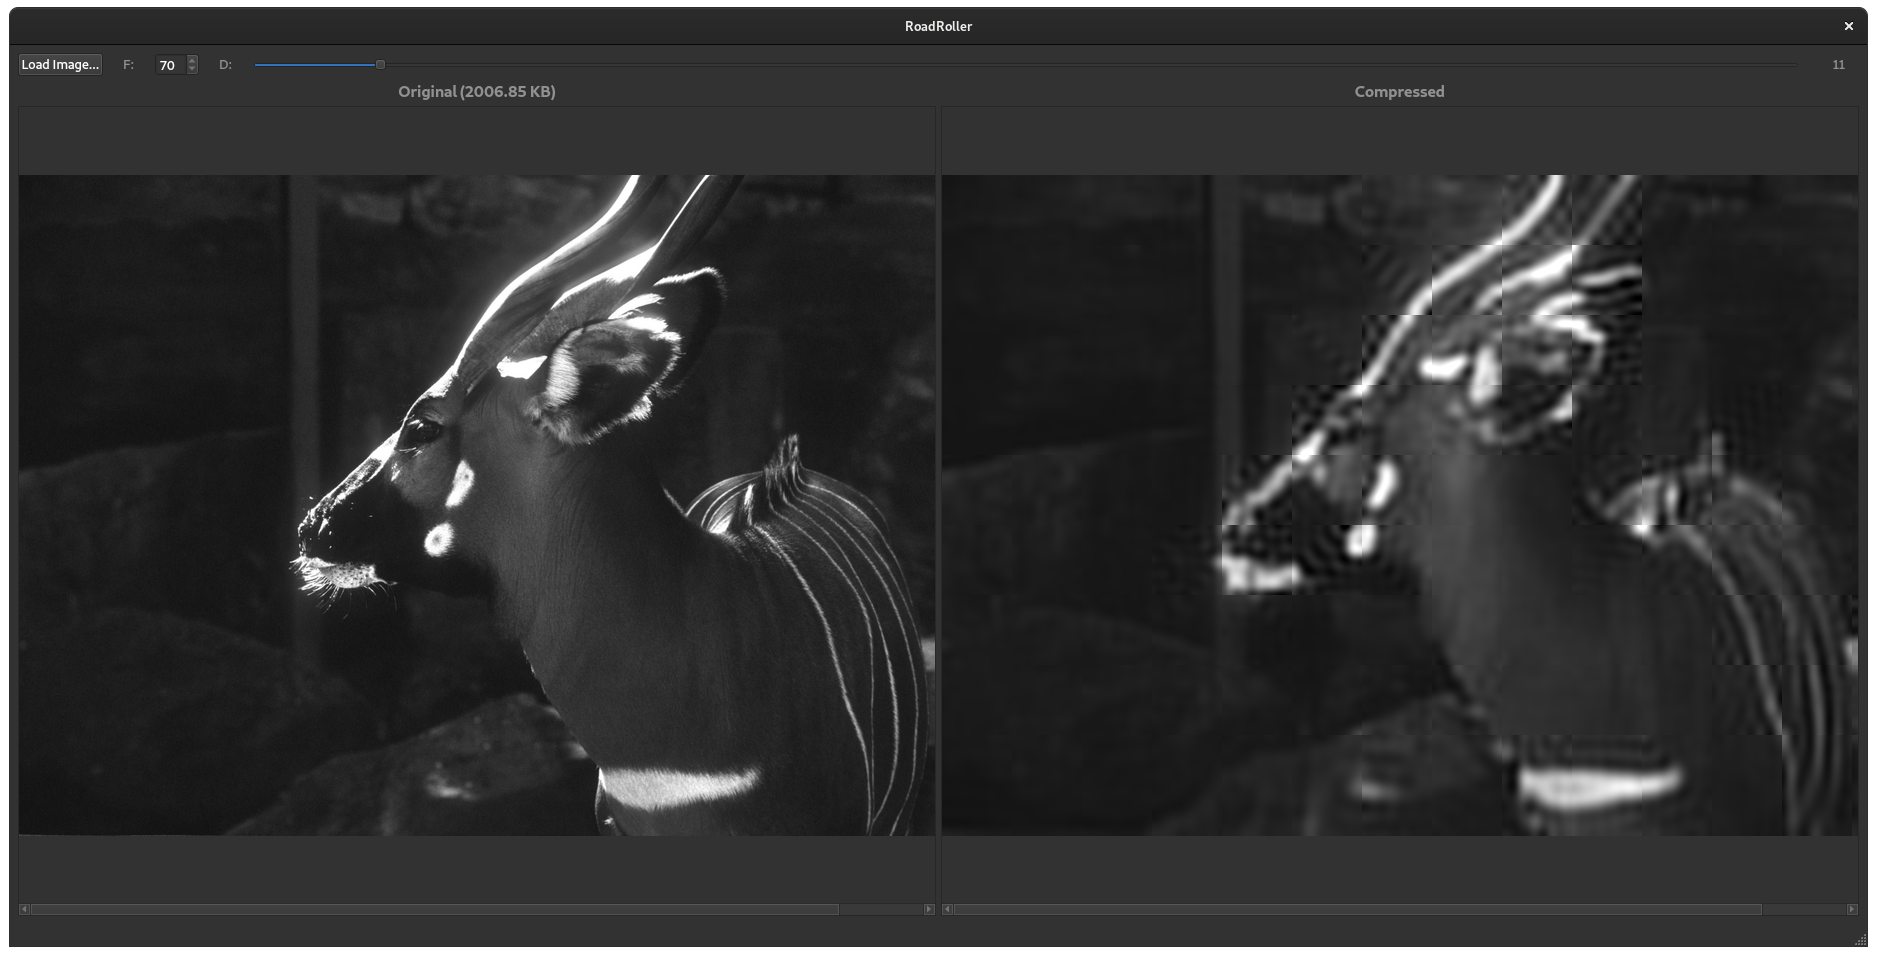
\includegraphics[width=1\linewidth]{figures/qt_deer}
	\caption{Programma di compressione basato su Qt}
	\label{fig:deer}
\end{figure}

Il diagramma delle classi relativo a questo progetto è molto breve, infatti sono state create solamente 2 classi. La prima per gestire l'interfaccia grafica, chiamata \textit{MainWindow}, mentre la seconda, \textit{BlockManager}, si occupa della gestione dei blocchi e la loro relativa compressione. Questo diagramma viene mostrato in Figura \ref{fig:class_diagram}.

\begin{figure}[h]
	\centering
	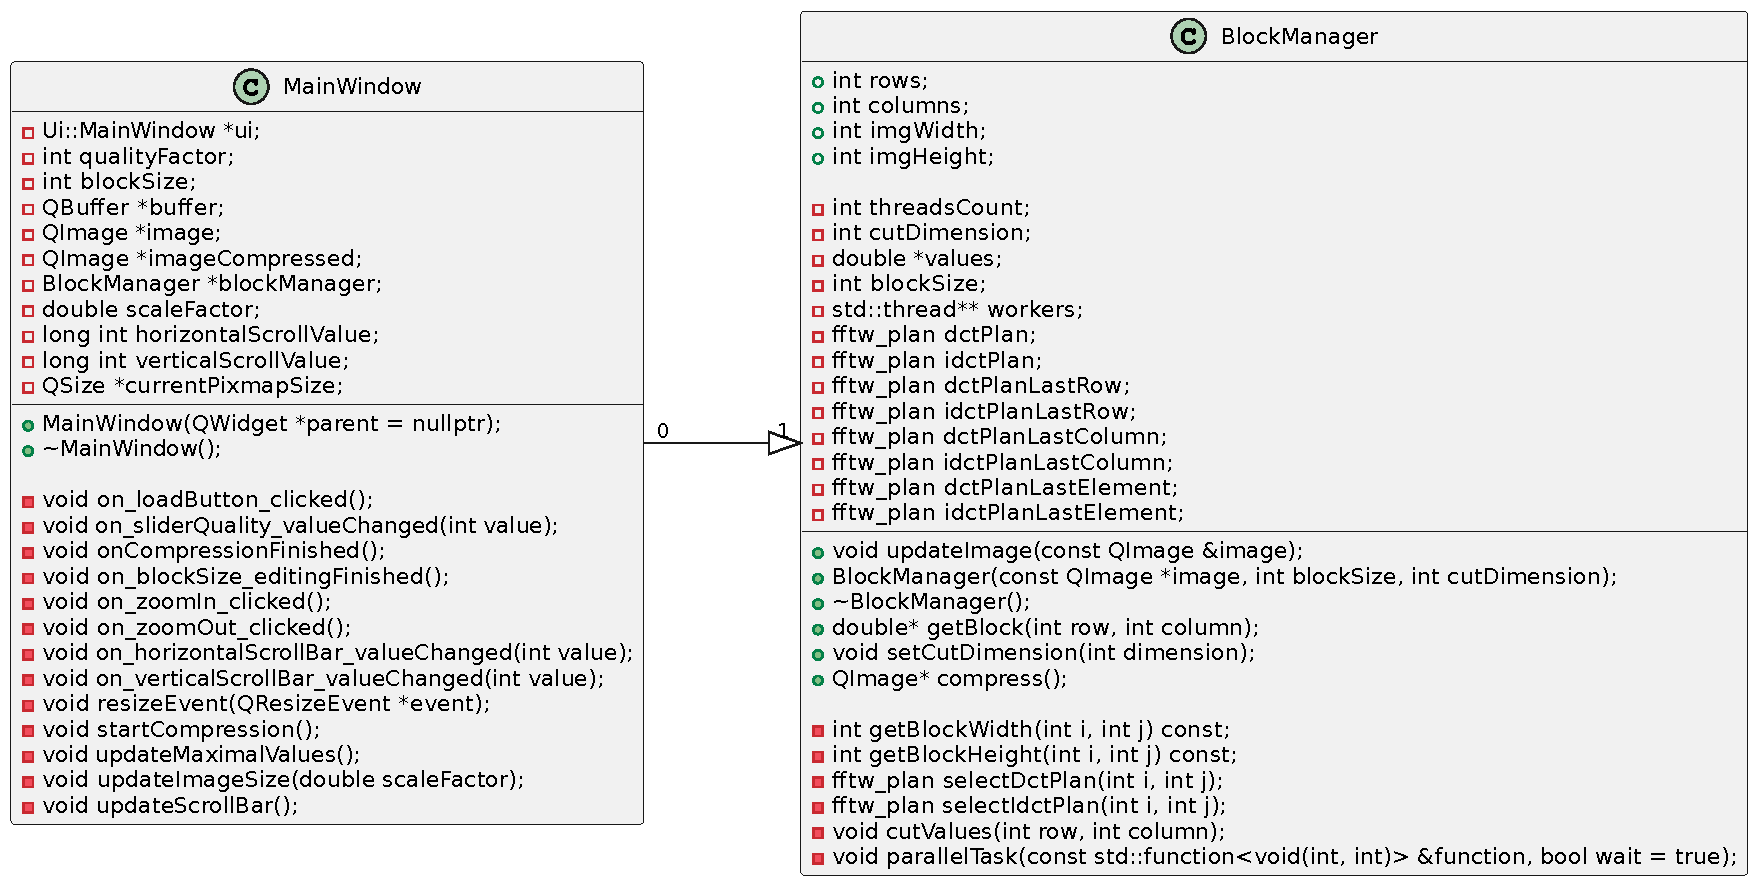
\includegraphics[width=1\linewidth]{figures/class diagram}
	\caption{Diagramma delle classi}
	\label{fig:class_diagram}
\end{figure}

\section{Features}

Alla versione base del progetto, descritto precedentemente, sono state aggiunte un insieme di funzionalità:

\begin{itemize}
	\item \textbf{Multithreading}: L'aggiunta dei thread permette una rapida compressione dell'immagine. Infatti essendo che i blocchi lavorano su aree della figura indipendenti gli uni dagli altri, è possibile eseguire le compressioni in parallelo, così come la scrittura dei pixel nell'oggetto immagine finale.
	
	Abbiamo fatto in modo che l'immagine venisse suddivisa in macroblocchi disgiunti tra loro, ognuno contenente un insieme di blocchi $F \times F$ dell'immagine. La cardinalità di questo insieme di macroblocchi è pari circa al numero di core/thread del processore su cui verrà eseguito il nostro programma di compressione. In questo modo, è possibile bilanciare il livello di parallelismo sulla base delle capacità della macchina di parallelizzare i task.
	\item \textbf{Navigazione dell'immagine}: All'interno dell'interfaccia grafica sono presenti degli slider e dei tasti per zoomare nelle immagine. Questi tasti sono sincronizzati in modo tale da poter visionare contemporaneamente le stesse zone delle 2 immagini. In questo modo si possono osservare più comodamente i vari effetti che la compressione comporta sulle immagini.
	\item \textbf{Aggiornamento in tempo reale}: Abbiamo costruito l'interfaccia grafica in modo che l'utente possa regolare e visualizzare in tempo reale la compressione dell'immagine, anche su zone particolari (ad esempio, dopo uno zoom). Grazie al parallelismo, inoltre, siamo riusciti a migliorare la latenza di questa operazione.
	\item  \textbf{Gestione dei bordi}:  A fini sperimentali, abbiamo provato ad implementare il processo di compressione in modo che venisse effettuata la DCT anche su blocchi di dimensioni inferiori, composti dagli scarti derivati dalla suddivisione in blocchi di dimensione $ F \times F$. Ulteriori informazioni su questa prova sono presenti alla Sezione \ref{sec:border}.
	
	\end{itemize}

\section{Gestione dei pixel in eccesso}\label{sec:border}

All'interno di questo progetto, abbiamo deciso in modo "sperimentale" di gestire in maniera leggermente diversa da jpeg i pixel sui margini.

Nello specifico, il nostro programma di compressione considera i pixel in eccesso derivati dalla suddivisione in blocchi e li utilizza per creare dei blocchi più piccoli, al fine di riempire l'intera immagine. Dopo questa operazione, ne esegue la DCT2 allo stesso modo degli altri blocchi. Prima di eseguire il taglio, però, la soglia di azzeramento delle frequenze viene adattata in modo da essere proporzionato alla minore quantità di frequenze e da rendere, quindi, la compressione dell'immagine più uniforme:

$$d' = \floor*{d  \sqrt{ \frac{W \cdot H}{F^{2}}}}$$

dove W e H rappresentano rispettivamente la larghezza e l'altezza del blocco preso in considerazione.
Inoltre, nel caso in cui $d'=0$, ma $d>0$, si mantiene il valore 1 al fine di evitare buchi indesiderati.

Abbiamo preso questa decisione perché, a differenza di jpeg, non siamo stati vincolati dalla matrice di quantizzazione e abbiamo potuto, quindi, sperimentare una gestione leggermente diversa del margine dell'immagine.


\begin{figure}
	\begin{minipage}{0.5\textwidth}
		\begin{center}
		
			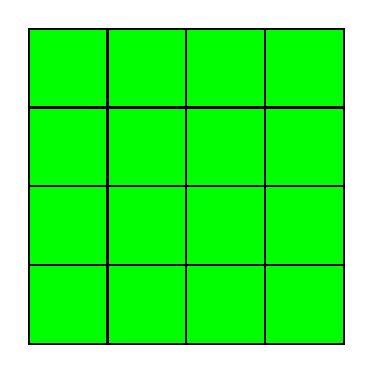
\begin{tikzpicture}
				[%%%%%%%%%%%%%%%%%%%%%%%%%%%%%%
				box/.style={rectangle,draw=black,thick, minimum size=1cm},
				]%%%%%%%%%%%%%%%%%%%%%%%%%%%%%%
				
				\foreach \x in {0,1,...,3}{
					\foreach \y in {0,1,...,3}
					\node[box, fill=red] at (\x,\y){};
				}
			
			
				\foreach \x in {0,...,3}{
					\foreach \y in {0,...,3} {
						\ifnumcomp{\x + (3 - \y)}{<}{5}{
							\node[box, fill=green] at (\x,\y){};
						}{};
					}
				}
				
				
			\end{tikzpicture}
		\end{center}
		\begin{center}
			(a)
		\end{center}
	\end{minipage}\hfill
	\begin{minipage}{0.5\textwidth}
		\begin{center}
			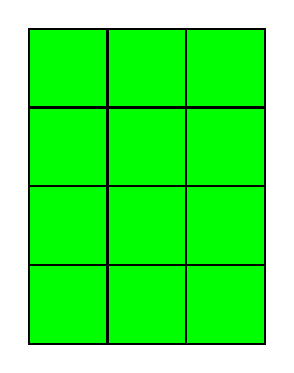
\begin{tikzpicture}
				[%%%%%%%%%%%%%%%%%%%%%%%%%%%%%%
				box/.style={rectangle,draw=black,thick, minimum size=1cm},
				]%%%%%%%%%%%%%%%%%%%%%%%%%%%%%%
				
				\foreach \x in {0,1,...,2}{
					\foreach \y in {0,1,...,3}
					\node[box, fill=red] at (\x,\y){};
				}
				
				
				\foreach \x in {0,...,2}{
					\foreach \y in {0,...,3} {
						\ifnumcomp{\x + (3 - \y)}{<}{5}{
							\node[box, fill=green] at (\x,\y){};
						}{};
					}
				}
				
				
			\end{tikzpicture}
		\end{center}
	\begin{center}
		(b)
	\end{center}
\end{minipage}
\caption{Taglio delle frequenze sulle diverse dimensioni dei blocchi}\label{fig:taglio}
\end{figure}

\section{Visualizzazione dei risultati}

Per mostrare meglio la compressione potremmo momentaneamente ignorare la conversione dei valori tramite la IDCT2. In figura\ref{fig:compression_values} viene mostrato il risultato ottenuto, dove è possibile osservare i coefficienti generati dalla DCT, i quali vengono successivamente tagliati per il valore di input scelto. In questo modo, ogni blocco conterrà dati diversi da 0 solo nella parte superiore del taglio, evidenziata anche graficamente dalla distribuzione del colore bianco nei singoli blocchi. Infatti tale tonalità rappresenta un valore elevato del coefficiente presente nella matrice, mentre le zone nere, rappresentano i valori che sono stati impostati a 0 dal taglio. Al fine di rendere migliore la visualizzazione, è stato temporaneamente modificato lo scaling delle DCT.

\begin{figure}[h]
	\centering
	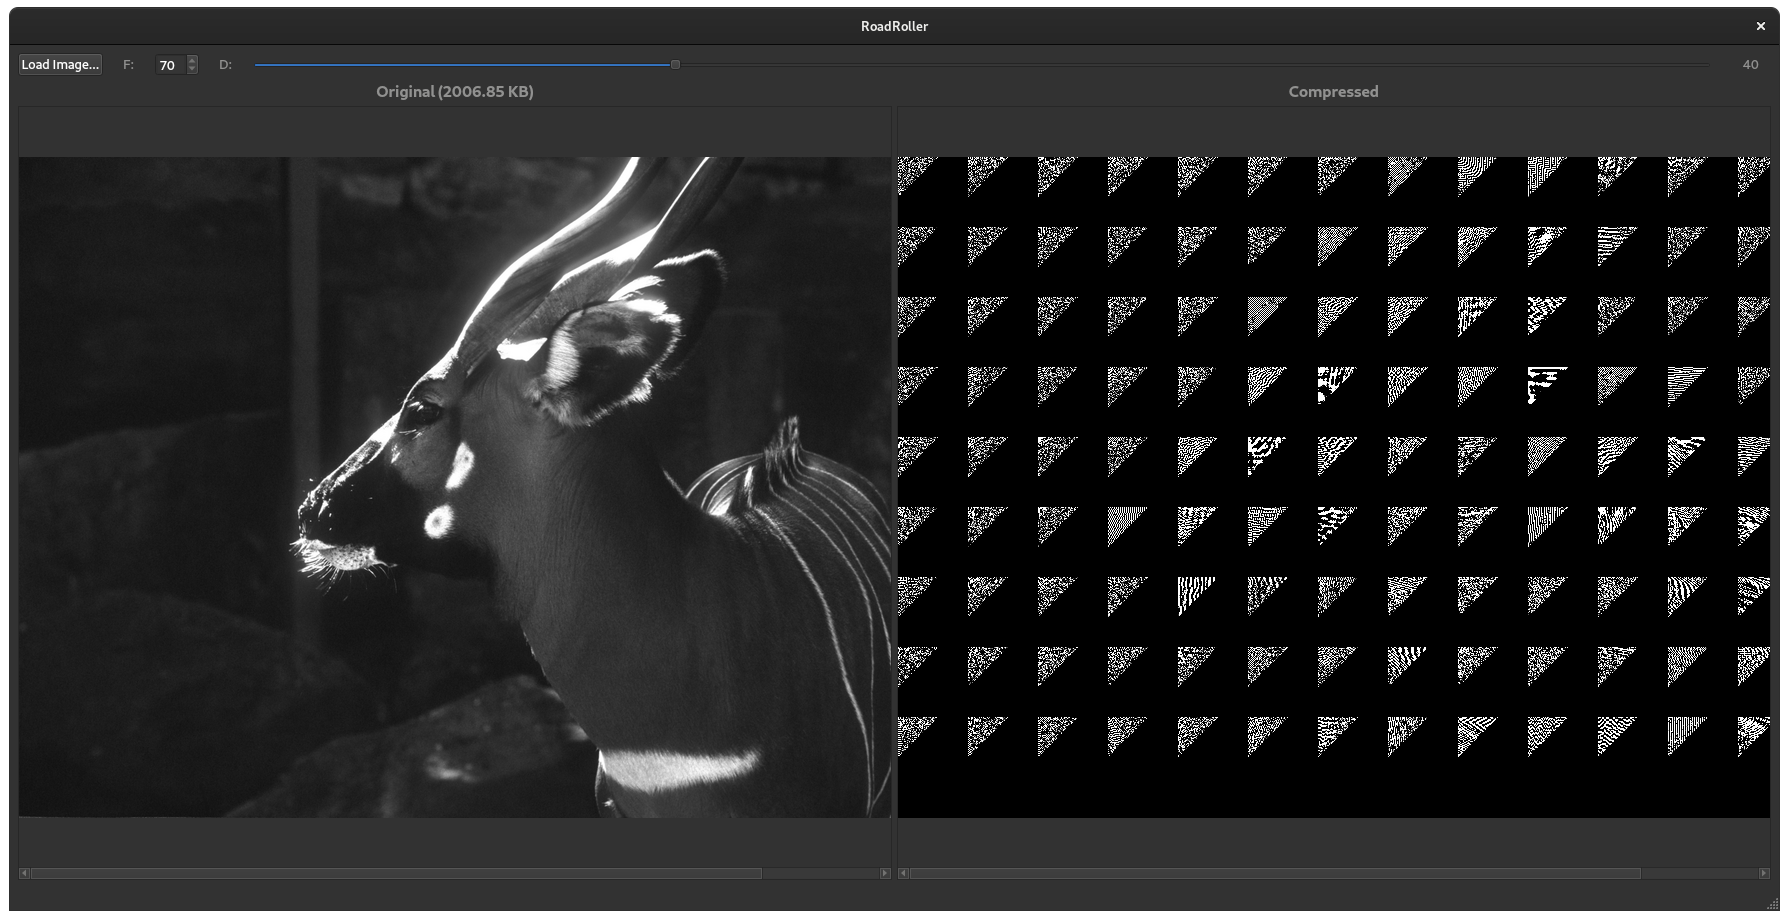
\includegraphics[width=1\linewidth]{figures/qt_dct_values}
	\caption{Valori della DCT generati dalla compressione (a meno dello scaling). Si noti il taglio netto delle frequenze determinato dalla soglia $d$.}
	\label{fig:compression_values}
\end{figure}

\subsection{Fenomeno di Gibbs}

Scegliendo un'elevata dimensione dei blocchi si rende particolarmente visibile il fenomeno di Gibbs, mostrato in Figura \ref{fig:gibbs}. La sua presenza tende ad essere più fastidiosa con blocchi grandi perché è più probabile che, all'aumentare di $F$, aumenta lo spazio all'interno del quale le basse frequenze cercano di compensare la carenza di quelle alte per rappresentare i cambiamenti repentini del tono di grigio presenti nel blocco stesso.

Nelle Figure \ref{fig:dct_values_on_gibbs} e \ref{fig:last_dct_values_gibbs} sono rappresentati rispettivamente l'intero istogramma del blocco mostrato in Figura \ref{fig:gibbs} e un suo zoom sulle ultime $50 \times 50$ frequenze. Nonostante la presenza di basse frequenze sia decisamente maggiore di quella delle alte frequenze, sono proprio quest'ultime che sono in grado di rappresentare al meglio i dettagli e, quindi, anche il bordo superiore della testa del cervo. Al momento del taglio, con un valore di $d$ basso, queste spariscono del tutto e non è, quindi, più possibile mostrare il cambiamento netto dell'immagine originale.

\begin{figure}[h]
	\centering
	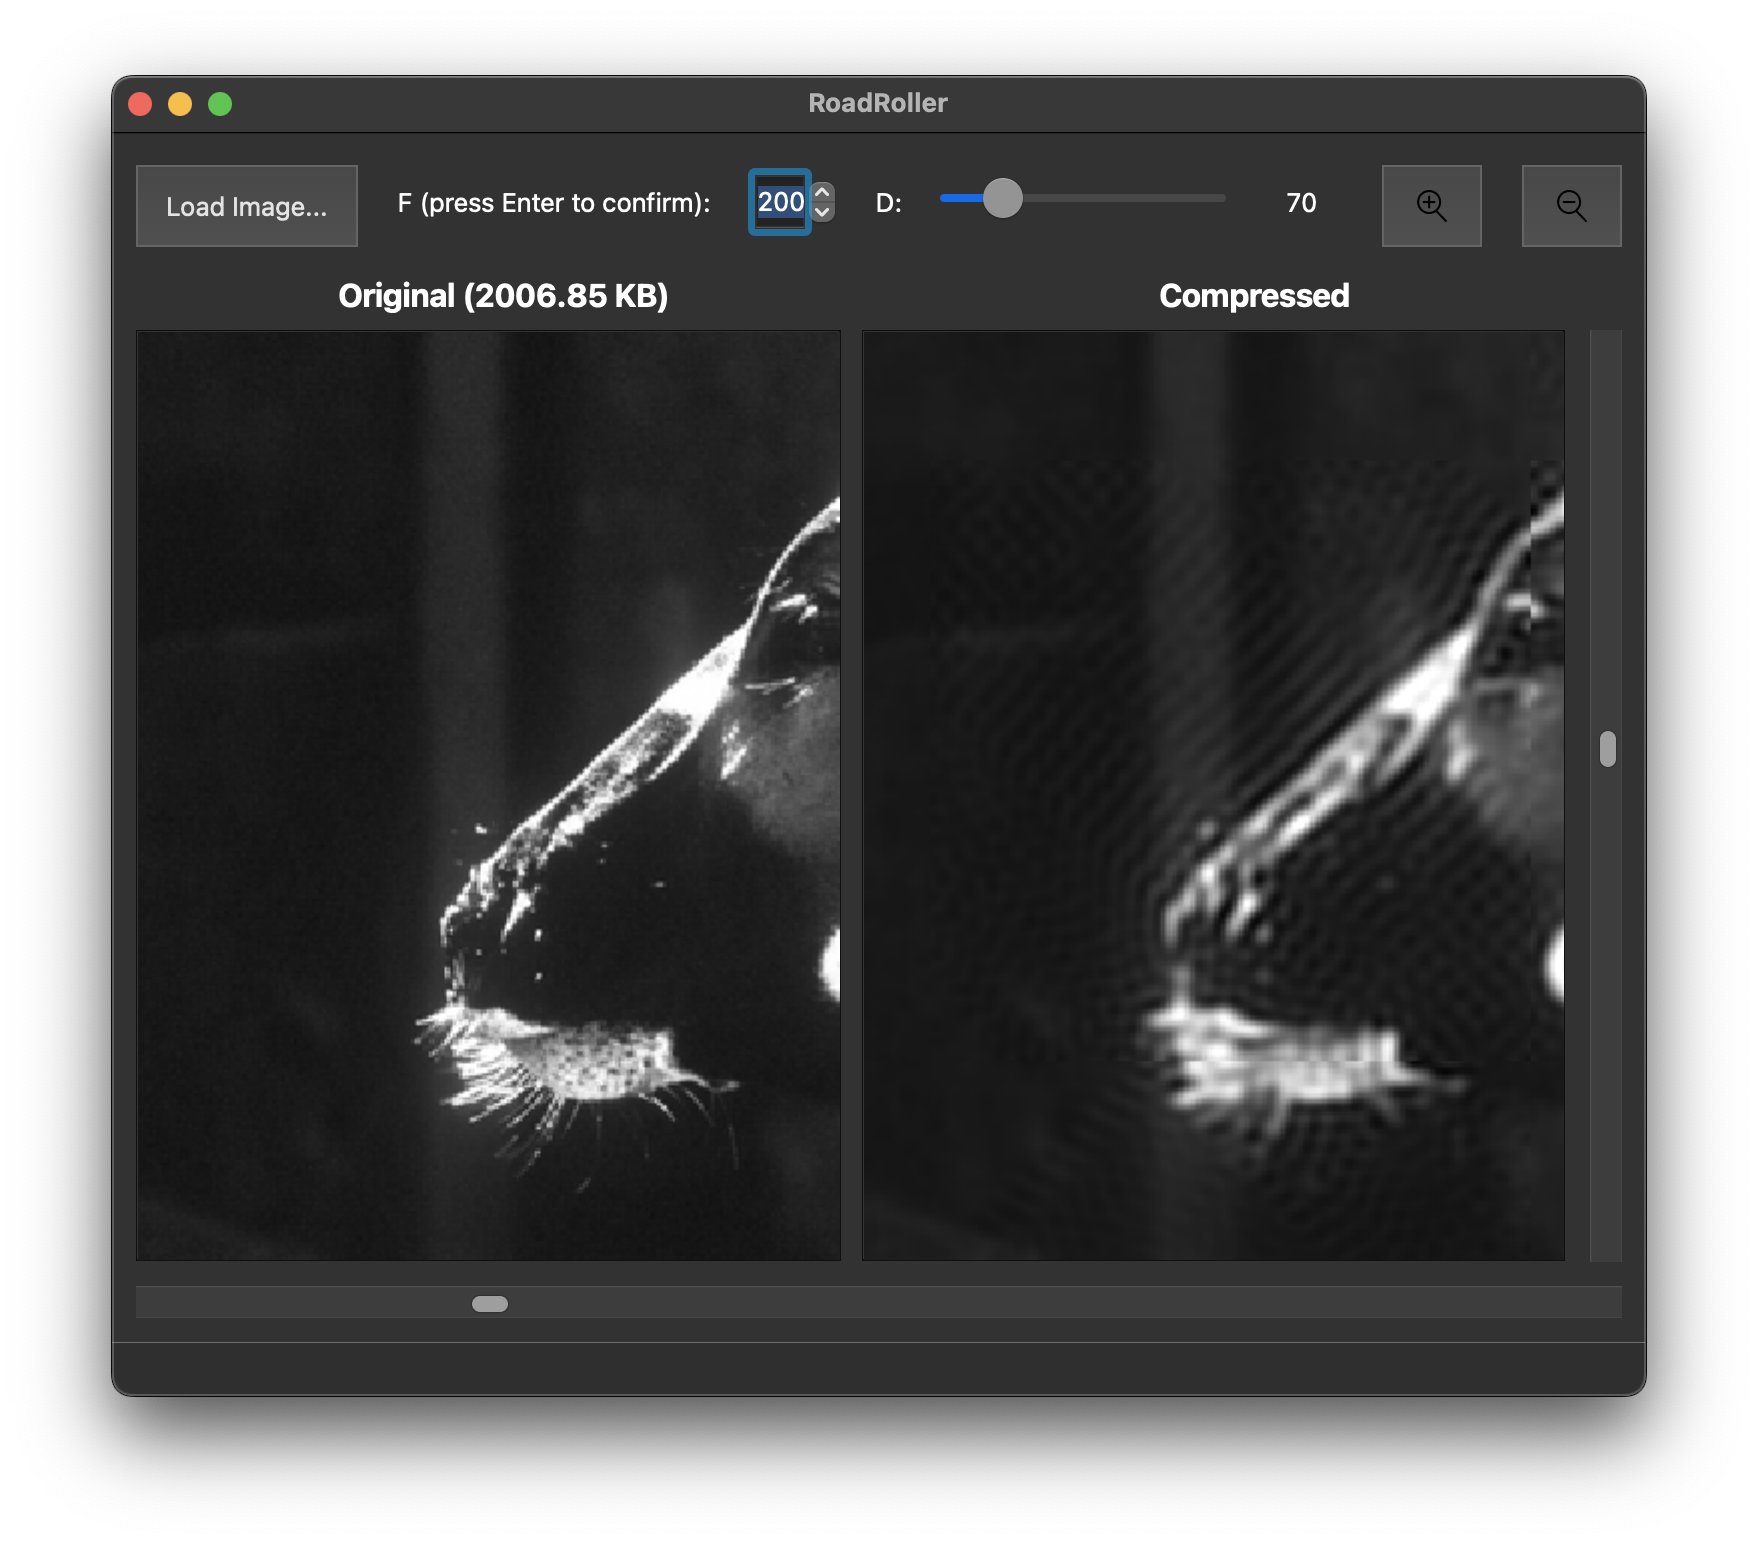
\includegraphics[width=1\linewidth]{figures/gibbs_phenomenon}
	\caption{Fenomeno di Gibbs su un blocco}
	\label{fig:gibbs}
\end{figure}


\begin{figure}
	\centering
	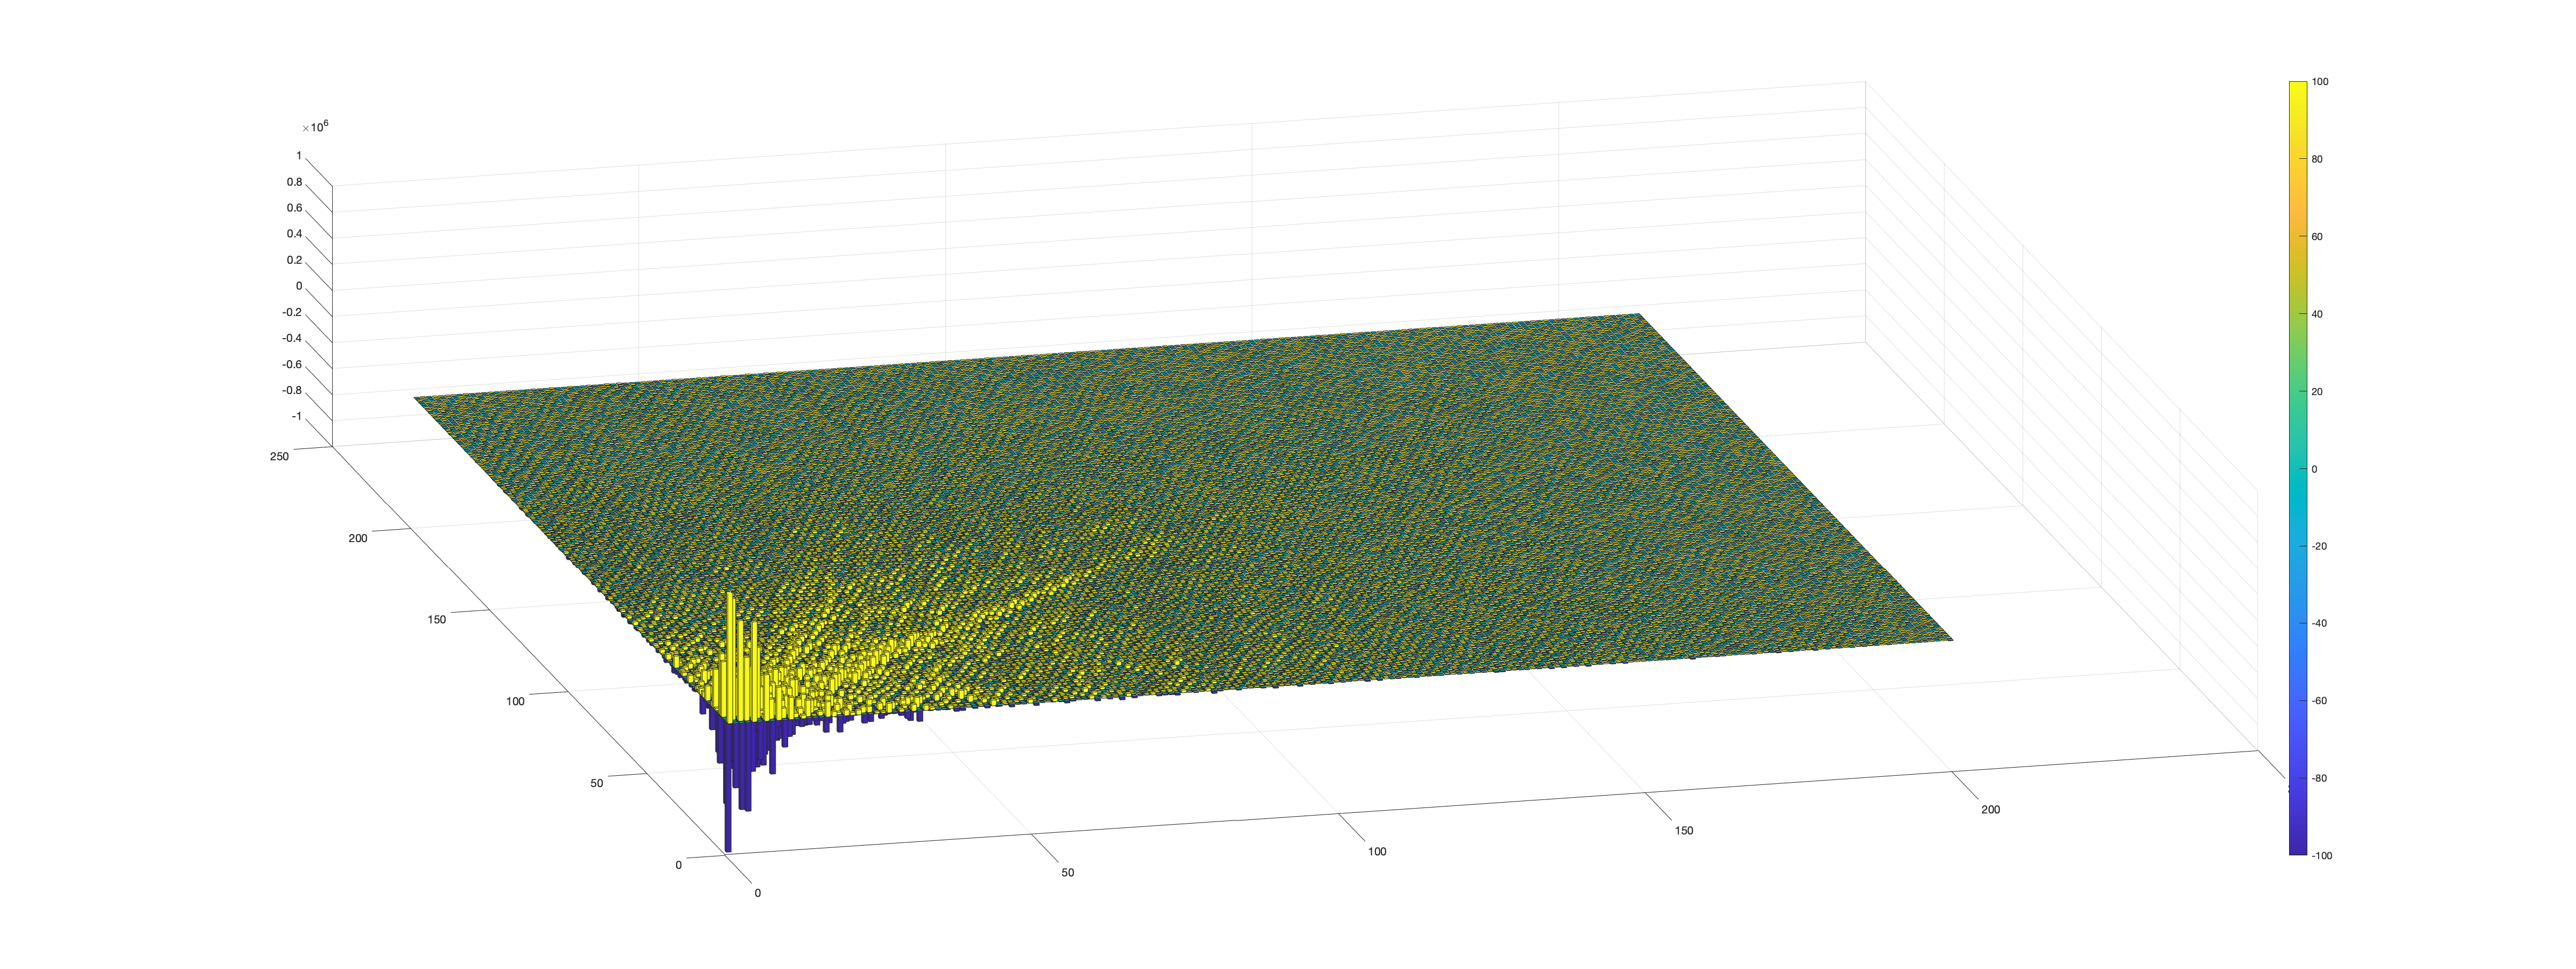
\includegraphics[width=1\linewidth]{figures/dct_values_3d.eps}
	\caption{Coefficienti DCT nel blocco mostrato in Figura \ref{fig:gibbs}}
	\label{fig:dct_values_on_gibbs}
\end{figure}

\begin{figure}
	\centering
	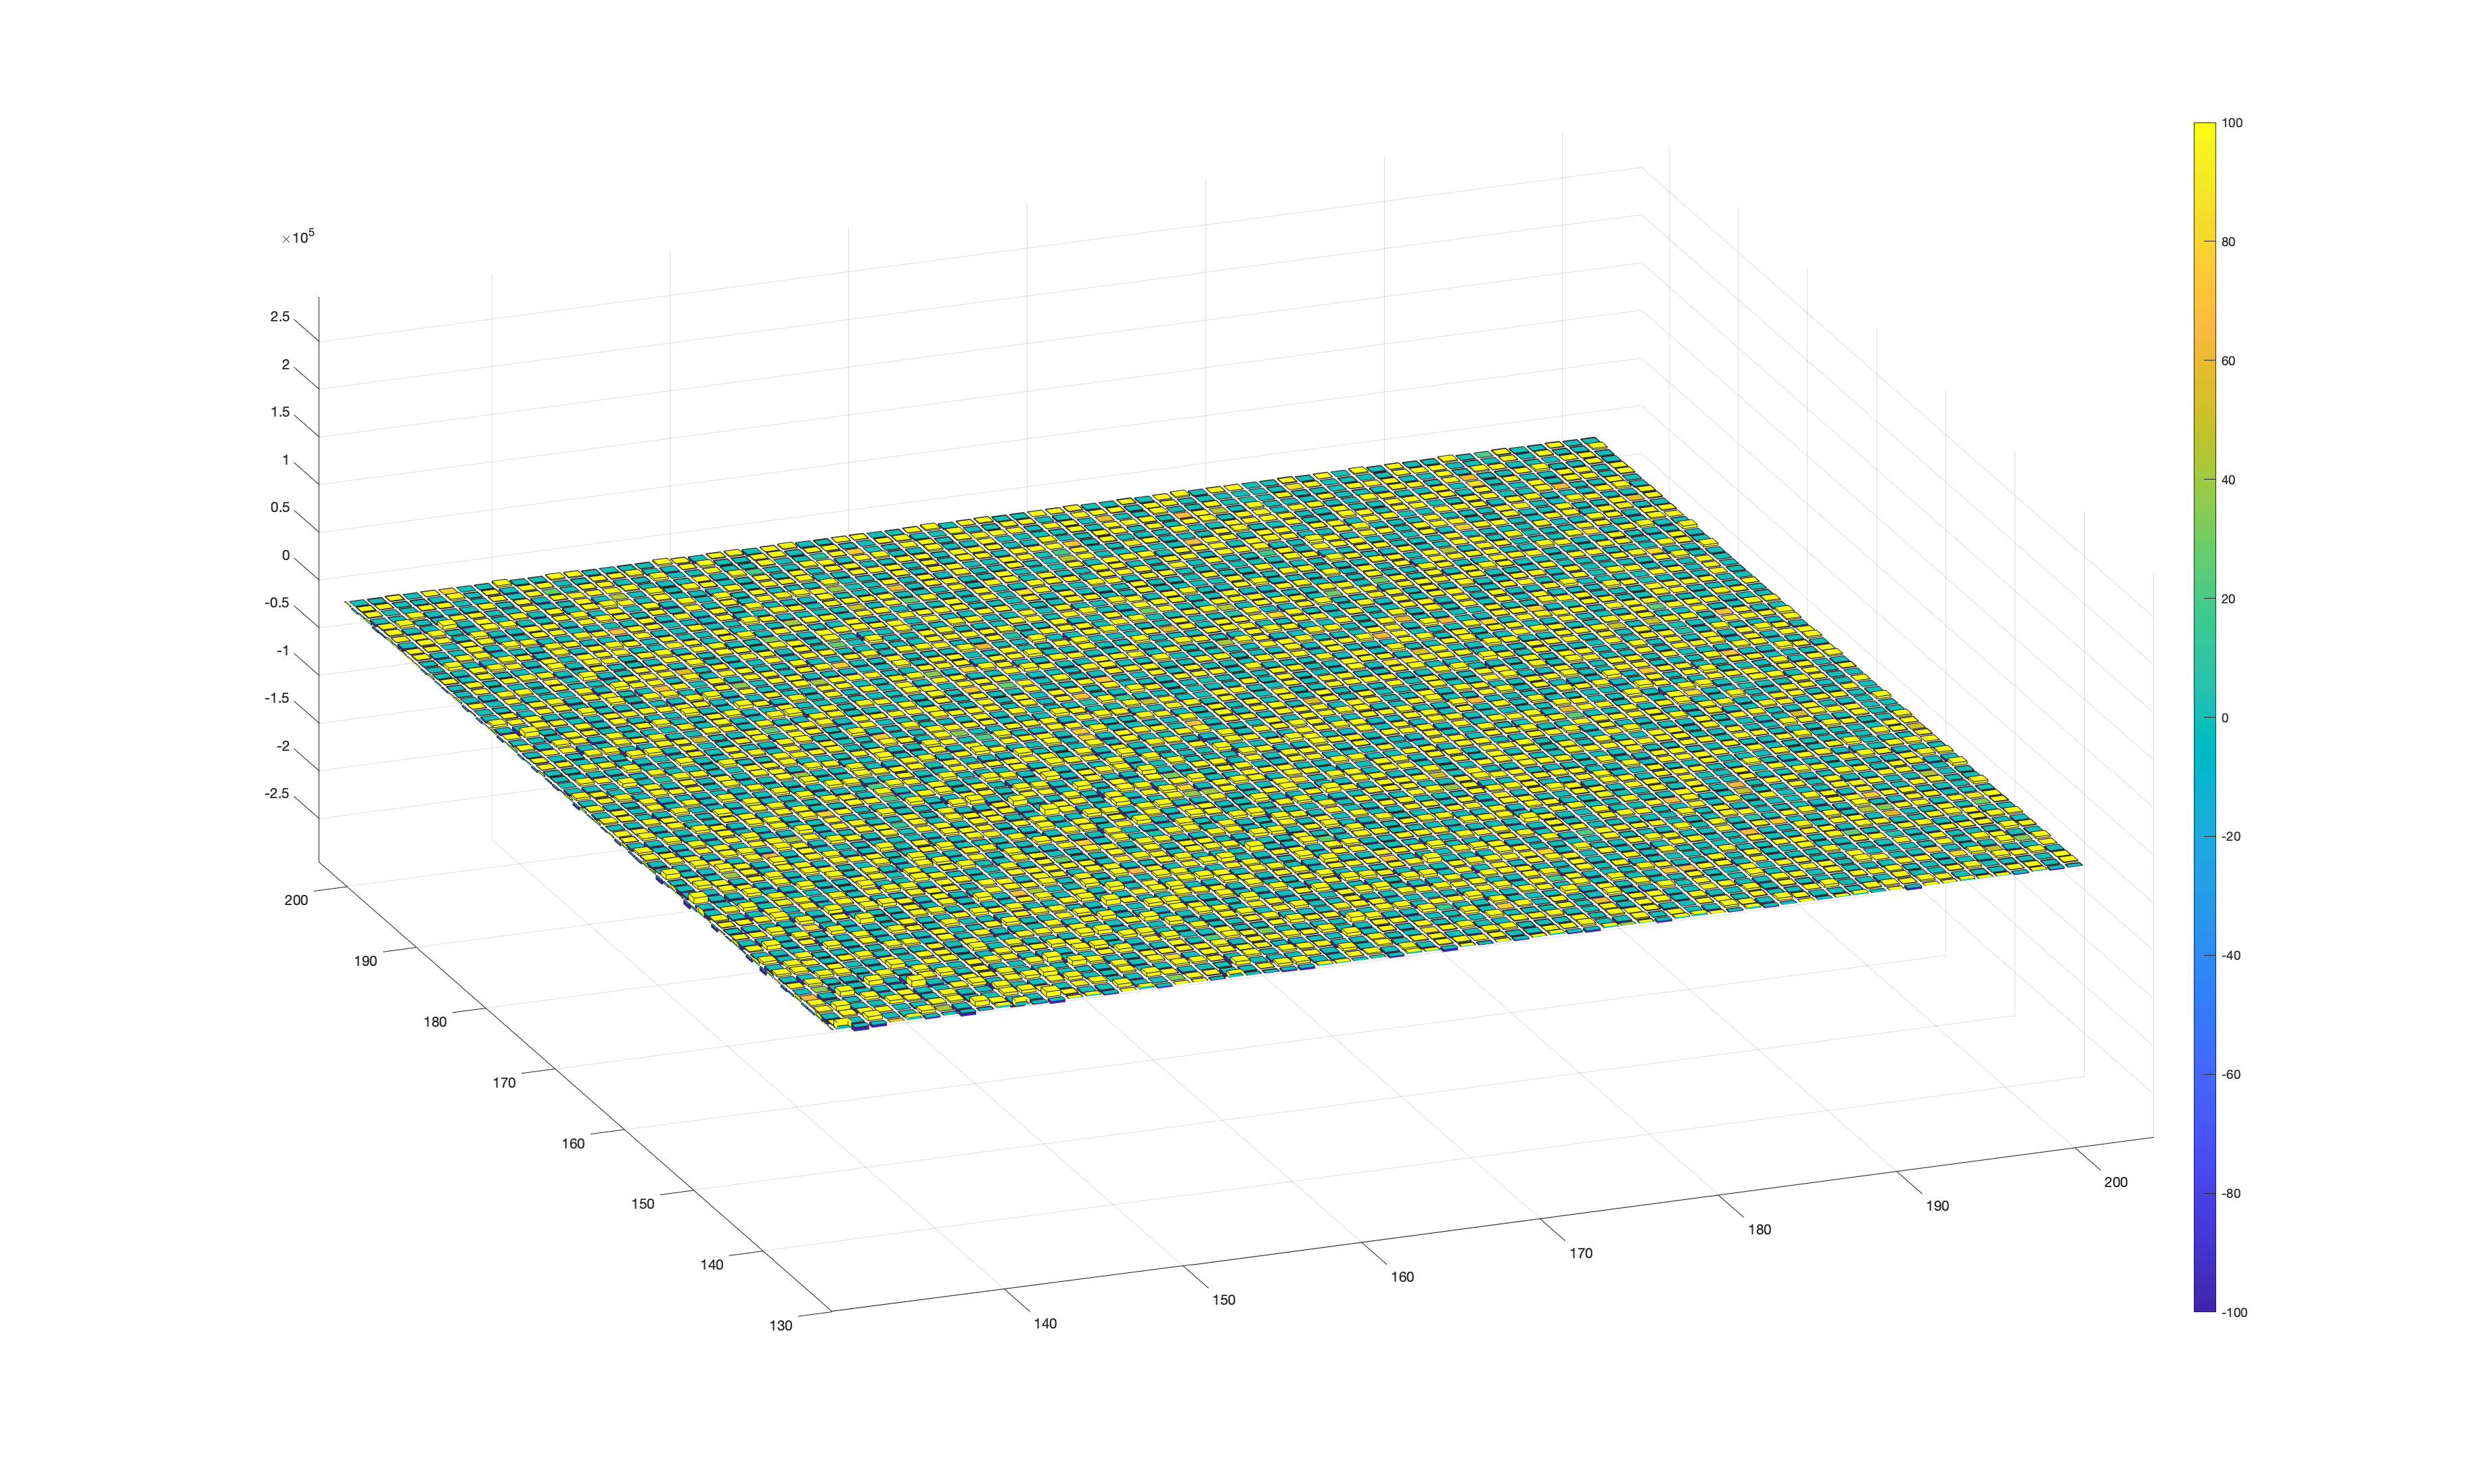
\includegraphics[width=1\linewidth]{figures/last_dct_values.eps}

	\caption{Ultimi 50 x 50 coefficienti della DCT relativi alla Figura \ref{fig:dct_values_on_gibbs}}
	\label{fig:last_dct_values_gibbs}
\end{figure}